% XCircuit output "mem_packet.tex" for LaTeX input from mem_packet.eps
\def\putbox#1#2#3#4{\makebox[0in][l]{\makebox[#1][l]{}\raisebox{\baselineskip}[0in][0in]{\raisebox{#2}[0in][0in]{\scalebox{#3}{#4}}}}}
\def\rightbox#1{\makebox[0in][r]{#1}}
\def\centbox#1{\makebox[0in]{#1}}
\def\topbox#1{\raisebox{-0.60\baselineskip}[0in][0in]{#1}}
\def\midbox#1{\raisebox{-0.20\baselineskip}[0in][0in]{#1}}
   \scalebox{1}{
   \normalsize
   \parbox{7.66667in}{
   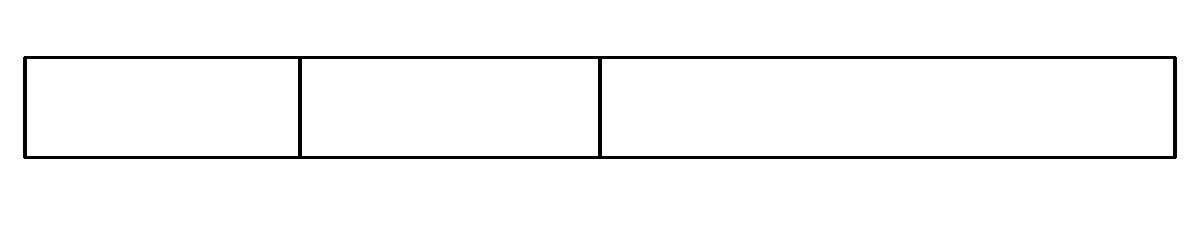
\includegraphics[scale=1]{mem_packet.eps}\\
   % translate x=960 y=150 scale 0.38
   \putbox{7.56in}{1.09in}{1.20}{0}%
   \putbox{0.06in}{1.09in}{1.20}{15}%
   \putbox{4.06in}{1.09in}{1.20}{7}%
   \putbox{3.56in}{1.09in}{1.20}{8}%
   \putbox{2.06in}{1.09in}{1.20}{11}%
   \putbox{1.56in}{1.09in}{1.20}{12}%
   \putbox{5.72in}{0.09in}{1.20}{asi}%
   \putbox{2.14in}{0.09in}{1.20}{number of bytes}%
   \putbox{0.64in}{0.09in}{1.20}{unused}%
   } % close 'parbox'
   } % close 'scalebox'
   \vspace{-\baselineskip} % this is not necessary, but looks better
